\documentclass[11pt]{scrartcl}
\usepackage{amsmath}
\usepackage{amssymb}
\usepackage[ngerman]{babel}
\usepackage[pdftex]{graphicx}
\usepackage{epstopdf}
\usepackage{hyperref}
\usepackage[utf8]{inputenc}
\usepackage{verbatim}
\usepackage{units}

\graphicspath{{./}{plots/}}

\title{VDVC Survey}
\author{Patrik Schönfeldt}
\date{\today}

\begin{document}
\maketitle

\textbf{Disclaimer:} Diese Arbeit wurde in der Absicht erstellt,
nützlich zu sein und neue und interessante Erkenntnisse zu gewinnen.
Auch wenn die Autoren einen wissenschaftlichen Hintergrund besitzen,
so können sie eine Qualität,
die ihren Maßstäben in ihren eigentlichen Fachbereichen genügt,
für dieses Freizeitprojekt allein zeitlich nicht gewährleisten.

\section{Beschreibung der Stichprobe}
Der erste Teil der VDVC-Umfrage (künftig: \emph{2013})
wurde über insgesamt 14 Tage
vom 23. Dezember 2013 bis zum 6. Januar 2014 durchgeführt.
1417 Personen haben diesen Teil abgeschlossen.
Der zweite und dritte Teil (künftig: \emph{2014} und \emph{2015})
wurde im Dezember 2014 bzw. 2015 durchgefüht,
die Zahl der komplett abgeschlossenen Fragebögen für diese Jahre beträgt 
1942 (2014) respektive 1356 (2015).
In jedem Jahr wurde bei den Communities \emph{For Uncut!},
\emph{Stigma-Videospiele/VDVC} und \emph{World of Players} für die Umfrage
geworben.
2014 ließ sich ein großer Anteil der Teilnehmer auf einen
Hinweis bei \emph{GameStar} und \emph{GamePro} zurückführen,
2015 gab es einen Hinweis vonseiten \emph{Electronic Arts}.

Da in jedem Jahr neu für die Umfrage geworben wurde und auch keine
Identifikaton der selben Teilnehmer über mehrere Jahre erfolgt,
ist eine statistische Betrachtung der Stichproben der Erhebungsjahre
geboten,
um Vergleichbarkeit zwischen den Jahren herzustellen und deren
statistische Abhängigkeit abschätzen zu können.
Außerdem kann die folgende Untersuchung
Aufschluss über die Repräsentativität der Umfrage geben.


\subsection{Altersstruktur}

\begin{figure}[htb]
	\centering
	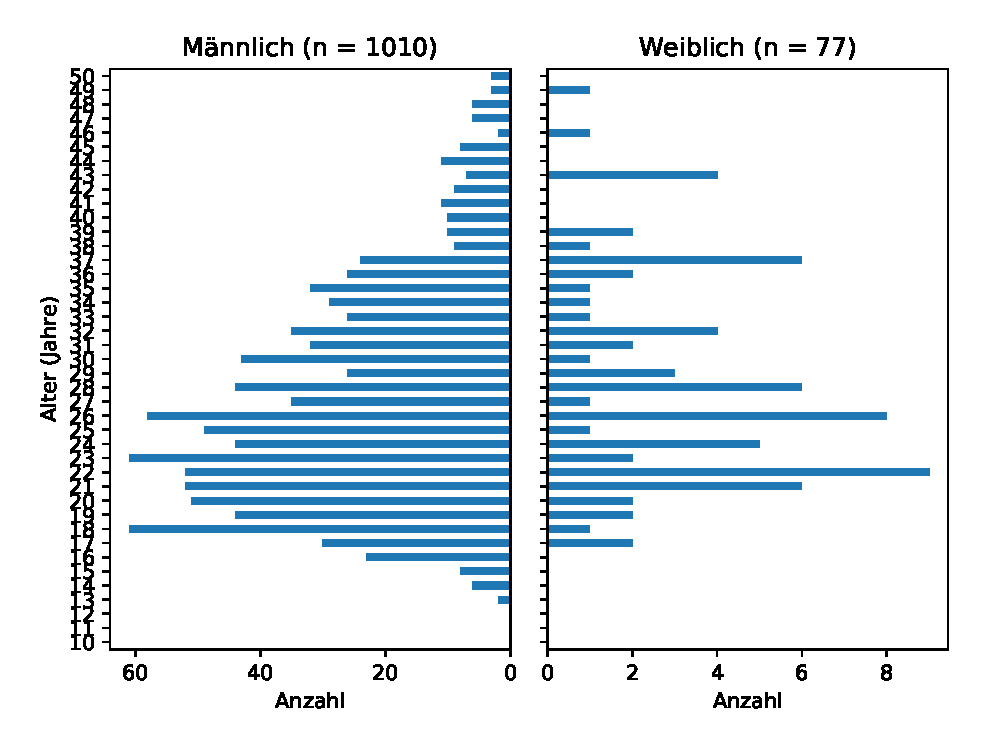
\includegraphics[width=15cm]{vgl/alter}
	\caption[Altersstruktur]
	{Altersstruktur des Teilnahmefelds.}
	\label{fig: alter}
\end{figure}

Die Altersstruktur (Abb.~\ref{fig: alter}) folgt über
den kompletten Erhebungszeitraum einem	ähnlichen Muster:
Jeweils gibt es kaum Teilnehmer unter 15 Jahren,
ab 18 Jahren erreicht die Verteilung ein Plateau.
Zwischen 40 und 50 Jahren sind nur wenige, noch älter kaum noch Teilnehmer.
Es ist im Laufe der Untersuchung eine leichte Verschiebung hin zu höherem
Alter zu beobachten, die jedoch weniger als ein Jahr pro Jahrgang der Umfrage
beträgt.


\subsection{Geschlechter}

\begin{figure}[htb]
	\centering
	\includegraphics[width=0.33\linewidth]{2013/geschlecht-rel}\hfill
	\includegraphics[width=0.33\linewidth]{2014/geschlecht-rel}\hfill
	\includegraphics[width=0.33\linewidth]{2015/geschlecht-rel}
	\caption{Geschlechter}
	\label{fig: geschlecht}
\end{figure}

Die Geschlechterverteilung (Abb.~\ref{fig: geschlecht})
zeigt einen deutlichen Überhang bei männlichen Teilnehmern.
Ihr Anteil beträgt \(\unit[94.0\pm1.6]{\%}\),
gegenüber \(\unit[5.4\pm1.4]{\%}\) bei den weiblichen Teilnehmern.
Wir gehen davon aus, dass diese Verteilung mehr oder weniger repräsentativ
für das untersuchte Milieu, den Kreis der \emph{Coregamer} ist.


\subsection{Einstiegsalter}

\begin{figure}[htb]
	\centering
	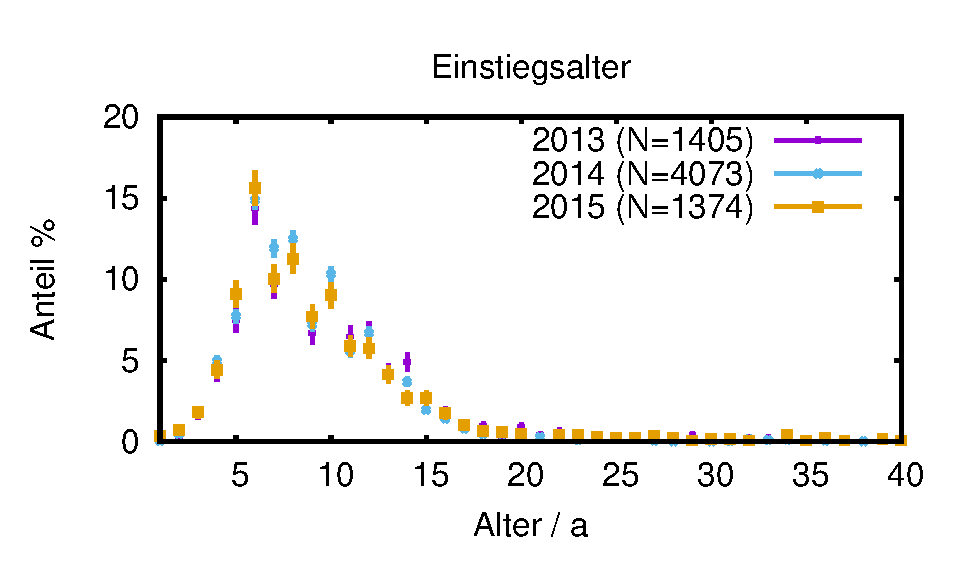
\includegraphics[width=15cm]{vgl/einstiegsalter}
	\caption[Einstiegsalter]
	{Einstiegsalter des Teilnahmefelds.}
	\label{fig: einstiegsalter}
\end{figure}

Der erste Kontakt mit Videospielen (Abb.~\ref{fig: einstiegsalter})
erfolgte bei der Hälfte der Teilnehmer im Alter von fünf bis zehn Jahren.
Mit einem Anteil von 15\% (konstant über alle Jahre der Erhebung)
gibt es im siebten Lebensjahr ein signifikantes Maximum.
Weitere Abweichungen von einem recht glatten Verlauf sind um das elfte
Lebensjahr zu beobachten.
Der Verlauf lässt sich mutmaßlich durch die Einschulung und durch den
Wechsel der Schulform erklären, der in diesem Alter üblich ist.



\subsection{Spielzeit}

\begin{figure}[htb]
	\centering
	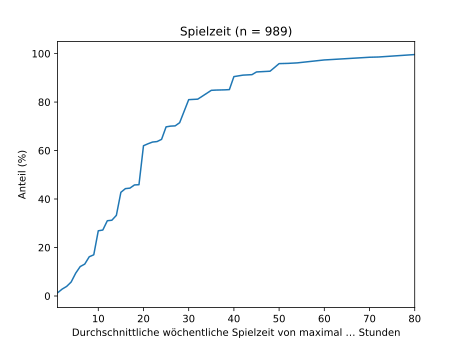
\includegraphics[width=15cm]{vgl/spielzeit}
	\caption[Spielzeit]
	{Tägliche Spielzeit des Teilnahmefelds.}
	\label{fig: spielzeit}
\end{figure}

Die tägliche Spielzeit (Abb.~\ref{fig: spielzeit})
folgte in allen Jahren der Erhebung einem ähnlichen Muster:
Weniger als eine Stunde und mehr als neun Stunden pro Tag
sind jeweils die absolute Ausnahme,
üblich (etwa 70\% der Befragten) sind ein bis fünf Stunden,
wobei die Verteilung etwa symmetrisch um das Maximum von knapp drei
Stunden ist.
Man beachte, dass nach einem Durchschnittswert gefragt war,
also auch das Wochenende berücksichtigt werden muss.
Die durchschnittliche Nutzungsdauer war bei der Umfrage 2014 geringer
als in den übrigen zwei Jahren,
was auf einen schwankenden Anteil an extremen Spielzeiten
zurückgeführt werden kann.
So gab es 10\% Wenigspieler (maximal eine Stunde am Tag) in 2013
12\% in 2014 und in 2015 nur 6\%,
für Vielspieler (über acht Stunden am Tag) lag die Quote dagegen bei
5\% (2013), 3\% (2014) und 6\% (2015)\footnote{Hier stellt sich die Frage,
ob pathologisches Verhalten indiziert ist oder ob durch den Erhebungszeitpunkt
-- hauptsächlich zwischen Weihnachten und Neujahr -- ein Bias erzeugt wurde.},
schwangt also in entgegengesetzter Richtung.



\subsection{Plattformen}

Ein wichtiges Merkmal von Gamern ist ihre bevorzugte Plattform.
Diese bestimmt nicht nur die Auswahl der zur Verfügung stehenden Spiele,
sondern ist insbesondere auch für die Erfahrungen mit Jugend- und
Verbrauchschutzthemen maßgeblich.
So haben die Anbieter der verbreitetsten Konsolen beschlossen,
keine jugendgefährdenden Inhalte vertreiben,
während diese am PC über das Internet zumindest teilweise erhältlich sind.




\subsection{Zusammenfassung}

Der teilnehmende Personenkreis ist über die Jahre nicht konstant geblieben.
Für diese Aussage sprechen schon die der Hinweise an verschiedenen Stellen
und die um Faktor Drei schwankende Teilnehmerzahl.
Dass insbesondere jüngere Personen hinzu kommen,
belegt die Entwicklung der Altersstruktur,
die sich pro Jahr der Erhebung weniger als ein Jahr zu höherem Alter bewegt.

Es ist davon auszugehen, dass es eine nicht vernachlässigbare
Zahl von Personen gibt,
die in mehreren Jahren einen Fragebogen ausgefüllt haben.
Aus diesem Grund können die Stichproben mehrerer Jahre
nicht als unabhängig angesehen werden.
Für die geplante Untersuchung von mehrjährigen Trends
ist die statistische Un-/ Abhängigkeit der Stichproben jedoch nicht von Relevanz,
solange Vergleichbarkeit besteht.

Die Konstanz der dargestellten Daten
über mehrere Jahre und Communities hinweg spricht für die
demographische Homogenität der hier abgebildeten Gruppe.
Wir definieren die `\emph{Coregamer} aus Deutschland'
über Spielenutzung und implizit (per Selbstselektion)
erfasste Identifikation mit Videospielen.
Gemäß der vorherigen Feststellung zur konstanten Zugehörigkeit
der Personen zu einer gemeinsamen Gruppe ist davon auszugehen,
dass unsere Umfrageergebnisse in Teilen denen
einer repräsentativen Abbildung der
\emph{Coregamer} aus Deutschland entsprechen.
Die Daten sind jedoch im Allgmeinen nicht repräsentativ
und insbesondere in keinem Fall repräsentativ für alle Gamer.


\section{Jugendschutz}

\subsection{Einsteigsalter}


\subsection{Verbreitung von Freigaben nach Alter}

Unterstellt man einen linearen Verlauf,
so lässt sich mittels Regression ermitteln,
wie stark die Verbreitung der jeweiligen Freigabestufen mit dem Alter
steigt oder fällt.
Die resultierenden Ausgleichsgeraden sind zusammen mit den Daten in
Abbildung~\ref{fig: freigabe-alter} dargestellt,
die dazugehörigen Werte finden sich in Tabelle~\ref{tab: freigabe-alter}.

\begin{figure}[htb]
	\begin{minipage}[b]{0.3\linewidth}
		\centering 2013 (n=3995)\\
		\includegraphics[width=\linewidth]{2013/freigabe-alter}
	\end{minipage}
	\hfill
	\begin{minipage}[b]{0.3\linewidth}
		\centering 2014 (n=13307)\\
		\includegraphics[width=\linewidth]{2014/freigabe-alter}
	\end{minipage}
	\hfill
	\begin{minipage}[b]{0.3\linewidth}
		\centering 2015 (n=4725)\\
		\includegraphics[width=\linewidth]{2015/freigabe-alter}
	\end{minipage}
	\caption{Verbreitung von USK-Freigaben nach Alter.
	Die Farben richten ich nach dem jeweiligen USK-Symbol:
	weiß=`ab 0', gelb=`ab 6', grün=`ab 12', blau=`ab 16', rot=`ab 18'.
	Zusätzlich geben schwarze Punkte Spiele an, die nicht bewertet wurden.}
	\label{fig: freigabe-alter}
\end{figure}

Es fällt auf,
dass USK6- und USK12-Titel beständig in höheren Altersgruppen beliebter
sind als bei jüngeren Umfrageteilnehmern.
Für USK18-Titel hingegen gilt das Gegenteil,
ihre Verbreitung nimmt mit dem Alter ab.
Bei USK0- und USK16-Titeln ist kein eindeutiger Trend erkennbar.

Es ist zudem zu beobachten,
dass der Anteil an nicht getesteten Spielen für alle Altersgruppen
über die Jahre größer geworden ist.
Wichtigster Grund hierfür ist die zunehmende Verbreitung von Indy-Games,
die oft keine Prüfung beantragen.

\newpage
\section{Anhang}

\begin{table}[ht]
\caption{Steigungen der Ausgleichsgeraden in Abb.~\ref{fig: freigabe-alter}.}
\label{tab: freigabe-alter}
\vspace{1em}
\centering
\begin{tabular}{r|c|r|c|r}
Jahr der Umfrage & Freigabe	&	Steigung	& Unsicherheit & P(falsches Vorzeichen)\\
\hline
2013 & USK00 & -0.02 & 0.12 & \(\unit[ 43,4]{\%}\)\\
	 & USK06 &  0.42 & 0.11 & \(\unit[ 10,1]{\%}\)\\
	 & USK12 &  0.30 & 0.22 & \(\unit[  8,6]{\%}\)\\
	 & USK16 & -0.07 & 0.19 & \(\unit[ 35,6]{\%}\)\\
	 & USK18 & -0.62 & 0.32 & \(\unit[  2,6]{\%}\)\\
\hline
2014 & USK00 &  0.01 & 0.06 & \(\unit[43,4]{\%}\)\\
	 & USK06 &  0.16 & 0.04 & \(\unit[<0,1]{\%}\)\\
	 & USK12 &  0.24 & 0.11 & \(\unit[ 1,5]{\%}\)\\
	 & USK16 &  0.14 & 0.11 & \(\unit[10,1]{\%}\)\\
	 & USK18 & -0.49 & 0.10 & \(\unit[<0,1]{\%}\)\\
\hline
2015 & USK00 &  0.40 & 0.19 & \(\unit[ 1,8]{\%}\)\\
	 & USK06 &  0.24 & 0.06 & \(\unit[<0,1]{\%}\)\\
	 & USK12 &  0.25 & 0.21 & \(\unit[11,7]{\%}\)\\
	 & USK16 & -0.28 & 0.21 & \(\unit[ 9,1]{\%}\)\\
	 & USK18 & -0.32 & 0.24 & \(\unit[ 9,1]{\%}\)\\
\end{tabular}
\end{table}


\clearpage
\bibliography{VDVC-Survey}{}
\bibliographystyle{alpha}

\end{document}
